\documentclass[UKenglish]{svproc}

% Localisation
\usepackage{babel}
\usepackage{csquotes}

% Bibliography
\usepackage[alldates=long, sorting=none]{biblatex}
\addbibresource{rubik_f.bib}

% Misc.
\usepackage{amsmath}
\usepackage[export]{adjustbox}
\usepackage{wrapfig}
\usepackage{subcaption}
\usepackage{float}
\usepackage{textcomp}

% URLs
\usepackage{url}
\urlstyle{rm}

% Hyperlinks (load last)
\usepackage[hidelinks]{hyperref}

%%% Project Information

\title{Rubik's Cube: Artificially Intelligent Solvers}
\subtitle{CS7IS2 Project (2020/2021)}
\author{
  William O'Sullivan   \and
  Basil Contovounesios \and
  Talha Ijaz           \and
  Fionnt\'an \'O Suibhne}
\institute{\email{
    wosulliv@tcd.ie,
    contovob@tcd.ie,
    ijazm@tcd.ie,
    suibhnef@tcd.ie}}
\authorrunning{O'Sullivan, Contovounesios, Ijaz, \'O Suibhne}

\begin{document}

\mainmatter
\maketitle              % typeset the title of the contribution

\begin{abstract}

An investigation into solving Rubik's Cubes by applying the following AI strategies was performed:
\begin{itemize}
    \item Genetic Algorithms (GA)
    \item Deep Reinforcement Learning + A$^{\ast}$ Search (DRL + A$^{\ast}$)
    \item Simulated Annealing (SA)
\end{itemize}
These approaches were used in order to determine solutions to a $2\times 2\times 2$ ($n=2$) ``Pocket Cube'' and a classic $3\times 3\times 3$ ($n=3$) Rubik's Cube.

The techniques broadly met with success, with every technique achieving a solution for a randomised cube. Times taken to solve each configuration varied between each instance, as did the number of turns required by each method to reach a solution. The DRL + A$^{\ast}$ method required the most up-front time due to its training component, but it 
%Can discuss #of turns taken to solve, time to solve, etc.


\keywords{genetic algorithms, deep reinforcement learning, simulated annealing}

%The abstract should summarize the contents of the report and should contain at least 70 and at most 150 words. It should be set in 9-point font size and should be inset 1.0 cm from the right and left margins. There should be two blank (10-point) lines before and after the abstract. This document is in the required format. The abstract should give a concise overview of the main points of the report: the motivation behind the work, a very high level description of the problem and how it was solved by the proposed algorithms. The abstract must not include any figures or table.

\end{abstract}
%
\iffalse
This document is a guideline for writing the final report for the CS7IS2 module Artificial Intelligence. You should follow its general structure as shown below.
You should not change its format (font, size, margin, space, etc.). 
Your report should be between 8 and 10 pages. Report that not comply to the format or exceed the maximum length will be penalised (-5 marks).
Brevity is desirable in communication, however you should provide all those details necessary for the good understanding of the described methods and algorithms. 

The report will be graded on the basis of:

\begin{itemize}
\item Originality - 10\%;
\item Technical soundness - 20\%;
\item Organisation - 20\%;
\item Clarity of presentation - 20\%;
\item Adequacy of bibliography/Results - 10\%
\item Presentation slides and recording) - 20\%
\end{itemize}





Your report should provide a survey and an experimental comparison of multiple solution approaches to a particular problem. This is a critical review of at least three papers that significantly contributed to advance the state-of-the-art for the problem you are analysing. It should not be a mere summary of the papers. You are expected to conduct an analytical review of the methods under analysis to try to find common aspect and differences, connections between methods, drawbacks and open problems. Unless the faced problem has emerged recently, students should choose their papers by diversifying the range of approaches used to solve the problem. A good guideline could be to choose a paper from a decade or two ago, and a couple of more recent papers. You need to experimentally evaluate approaches in a simulation of a problem, in a range of scenarios, and analyse the pros and cons of each approach. 
\fi

\section{Introduction}
%WRITING HERE
\subsection{Motivation}
1974 saw many historical events, including the election of the first female President of Argentina and ABBA's victory at the Eurovision with their iconic hit ``Waterloo''. 1974 also bore witness to the invention of the Rubik's Cube, a puzzle which has been in the minds of both pure mathematicians and computer scientists alike for decades. Whilst the puzzle has now been bested (even giving rise to the phenonmenon of Speedcubing!) it still serves as region of interest in fields where there is more concern for the method of solution.\\

Puzzles have long been a useful tool for examining the utility of artificial intelligence. Puzzles provide us with what would be considered an intellectual challenge, and creating agents that can produce solutions to puzzles can give us greater insight into both the limitations of such intelligences, as well as their strengths highlighting key areas where AI may find further use.

In the specific case of this investigation, we examine different agents for the problem of solving a Rubik's Cube, or indeed its smaller cousin the $2\times 2\times 2$ Pocket Cube, which will generally be described in the same way as it is simply a variant with a smaller state space. This particular puzzle sits at a cross-roads in terms of analysis. The Rubik's Cube is by no means a trivial pathfinding algorithm owing to the importance of move order but neither is it a puzzle without a known solution. That said, the Rubik's Cube itself only represents one member of a family of similar puzzles, for example higher dimensional $2\times 2\times 2\times 2$ objects, or longer sided $4\times 4\times 4$ cubes. A number of researchers have spent time investigating different methods of solving the cube via these intelligent agents only for some to determine that their approach does not suit the Rubik's Cube, whilst others meet with successful solutions.

At the outset, it was not expected that all of the approaches would yield perfect solutions to the Rubik's Cube. The heart of the investigation is built around understanding the methods and their applications in order to solve problems of this type, and this report will endeavour to share those findings accordingly.

\emph{NOTE: INCLUDE ONE\_DRIVE LINK}


\iffalse
In this section, you should introduce your work: what are the motivations behind this work? What is the relevant problem that you are investigating? Why is it relevant? 
Briefly, introduce the background information required to understand the problem and the concepts that you will develop. 

This section should also contain the link to the recording of your presentation (college OneDrive link – please make sure sharing permissions are such that everyone with tcd email can access it)
\fi

\section{Related Work}
In keeping with the directive that the focus of the investigation should be on recent solutions of this field of problem, one group have been quite prolific in their publications on Rubik's Cube solvers in particular. The work of Stephen McAleer, Forest Agostinelli, Alexander Shmakov and Pierre Baldi~\cite{mcaleer2018solving, mcaleer2019solving, agostinelli2019solving} formed a consistent basis of understanding for the Rubik's Cube problem as a whole, whilst also drawing attention to the use of Deep Reinforcement Learning centred around their DeepCube solver. It was possible for the researchers to use the policies determined by DRL with different search approaches, including Monte Carlo Tree Search (MCTS) and A$^{\ast}$ Search.

Beyond the use of DRL, however, lay two other approaches which draw influence from biology and physics, in Genetic Algorithms and Simulated Annealing respectively.

Genetic Algorithms are a way of generating increasingly close approximations to a solution, to the point where a solution itself is achieved. The work of El-Sourani et al.~\cite{10.1007/978-3-642-12239-2_9} utilised GA to solve a Rubik's Cube by incorporating the analytical solution to a Rubik's Cube based on the original work by Thistlethwaite~\cite{Thistlethwaite}. Whilst this technique resulted in solutions for any given cube configuration, Smith et al.~\cite{10.1145/2908812.2908887} attempted to build on this by determining policies with their GA rather than determining configuration-unique solutions, ultimately meeting with a great degree of success.

Simulated Annealing is a kind of random search method not unlike the aforementioned MCTS, however it possesses an additional strength in that it is also an iterative improvement algorithm. This means that the SA approach is able to escape local extrema, whilst consistently improving performance. SA has seen use in solving Sudoku puzzles, as in the work of Lewis~\cite{SAarticle}, and indeed SA could be applied to solving Rubik's Cubes by tweaking how the cost function is determined.

Between the applications of DRL + MCTS, DRL + A$^{\ast}$, GA for values, GA for policies and SA, a decision was made to investigate the properties of DRL + A$^{\ast}$, GA for values, and SA.

DRL + A$^{\ast}$ was selected as an investigation into the most modern approach to solving Rubik's Cubes. GA for values would allow for investigation of the differences between performance on $n=2$ and $n=3$ cubes without the added complexity of trying to determine policies for the different sized cubes. Finally, SA was selected in order to examine the effects of stochastic solvers in Rubik's Cubes, which had been scarcely investigated.

Overall, the proposed techniques comprise a decent and broad collection, and draw on a diverse set of approaches to solve one popular problem.

It should be noted that an implementation~\cite{Shoukat2019} based the work of Korf~\cite{KORF198597} was used as a baseline for comparison in terms of runtime. It is important to note that this algorithm does rely on human (domain) knowledge however, and so acts not as a baseline to beat necessarily, but a good comparison between the agents which do not have human knowledge, and those that do.

%In this section you will discuss possible approaches to solve the problem you are addressing, justifying your choice of the 3 you have selected to evaluate. Also, briefly introduce the approaches you are evaluating with a specific emphasis on differences and similarities to the proposed approach(es).

\section{Problem Definition and Algorithm}
The Rubik's Cube for both $n=2$ and $n=3$ is a sparse state space problem, meaning that only one solution exists in an otherwise very large state space. This presents unique challenges to finding suitable techniques for devising solutions to the cubes.

\subsection{Deep Reinforcement Learning + A$^{\ast}$ Search}
Reinforcement Learning (RL) involves exploring state spaces in order to determine optimal policies for maximising rewards. In the case of a Rubik's Cube, the state space is incredibly sparse, with $\sim 10^{19}$ possible states, and only one solution. As such, classical RL is insufficient to solve a Rubik's Cube, leading to the requirement of DRL. DRL utilises Deep Learning which is able to combine and interpret information to reduce the overhead of exploring such a sparse state space. For example, rather than having to explore the more than a quintillion different states, the use of DRL can convert these collections of states into groups, from which the RL algorithm can then build policies more easily.

Unfortunately, even with these advanced techniques the Rubik's Cube proved unsuitable for solving with DRL alone. The sparse nature of the problem means that the learning element can often fail to find its way to a goal state from which it can claim a reward. To alleviate this problem, the way in which the DRL training occurs is changed; rather than starting with a randomised cube and trying to solve from there, a solved cube is randomised with the agent knowing how the cube achieved a solution from a seemingly random state. This is called Autodidactic Iteration, and ensures that every training instance can result in a solution. It is in this way that the inputs for the DRL can be selected to yield a useful basis for training. The resulting trained models then served as a heuristic to inform an A$^{\ast}$ Search technique in order to solve the Rubik's Cube.  In this sense, the trained Deep Neural Net (DNN) approximates an otherwise infeasibly large mapping of states to their respective values, i.e. their distance from the goal.

The other component of the A$^{\ast}$ cost function, the cost from the starting state, is often weighted to achieve better runtime performance.  In this investigation, the effects of varying this weight were examined, effectively demonstrating the relationship between a runtime-efficient and number-of-moves-efficient solution to different cubes.

\subsection{Genetic Algorithms}

\begin{figure}[!h]
\begin{small}
\centering
\linespread{1.0}
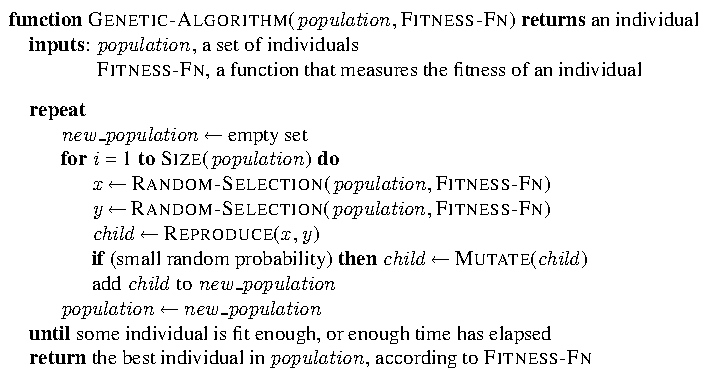
\includegraphics[width=0.9\linewidth]{images/genetic-algorithm}
\caption{Genetic Algorithms utilise reproduction, whereby a parent passes its characteristics onto its child. Over several generations an individual that better satisfies the fitness criteria emerges~\cite{10.5555/1671238}.}
\label{fig:fig0}
\end{small}
\end{figure}

The applications of GA to solve Rubik's Cubes in the literature were based on an analytical solution. The analytical solution broke the method into four distinct parts, based on human knowledge, and so the GA approach utilised these conditions as waypoints between the evolution of population. GA define populations as a set of approximate solutions, with each individual representing one such attempt. Certain individuals are better suited to meeting fitness criteria (i.e. how well a solution conforms to the required behaviour) and so upon the passage of a generation, individuals with better fitness have a higher probability to reproduce, creating a new individual with characteristics from two previous approximations. However, reproduction is not the only way in which the population evolves. Concepts of mutation and elitism allow for the propagation of individuals with desirable traits as well. Overall, the passage from one generation to the next is composed of 40\% offspring, 50\% by mutation and 10\% by elitism. Offspring come about based on the previous notion of reproduction, whilst mutants are the result of lone individuals experiencing a number of small move alterations, and elitism allows for the propagation of the portion of the population that was judged to be most fit. The elites are selected from the best population that did not produce offspring, as to give them another chance to reproduce.

The idea is that these new individuals will possess a combination of attributes that allow them to satisfy the fitness function even better, in turn increasing the chance of their characteristics being passed along. In this manner that mimics natural selection, over a number of generations it becomes possible to arrive at a population that contains individuals which satisfy the fitness criteria perfectly, at which point a solution has been reached.

In this investigation, GA were used to solve a Rubik's Cube without human knowledge. The analytical solution modified the fitness criteria at different stages, in accordance with the Thistlethwaite methods, such that the direction of evolution was modified to become increasingly adept at solving the Rubik's Cube in a low number of steps.  This particular implementation however did not alter the cost function at any point, and so the GA could only act to minimise the following cost function:
\begin{align*}
  \text{All elements of a row} &
  \begin{cases}
    +0 & \text{all colours uniform} \\
    +1 & \text{all colours not uniform}
  \end{cases} \\
  \text{All elements of a column} &
  \begin{cases}
    +0 & \text{all colours uniform} \\
    +1 & \text{all colours not uniform}
  \end{cases} \\
  \text{All elements of a face} &
  \begin{cases}
    +0 & \text{all colours uniform} \\
    +1 & \text{all colours not uniform}
  \end{cases}
\end{align*}
These cost conditions were used to calculate the cost on each face, which in turn were used to determine the cost of the overall cube. For example, whilst a cost~0 cube gives a completely solved system, a cost~12 cube implies that the cube may be at most a half-turn (180\textdegree) away from a solution.

\subsection{Simulated Annealing}

\begin{figure}[!h]
\begin{small}
\centering
\linespread{1.0}
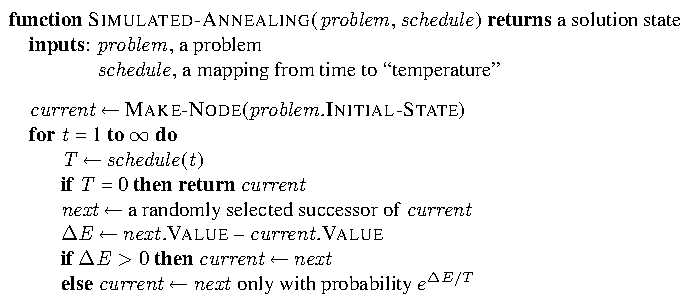
\includegraphics[width=0.9\linewidth]{images/simulated-annealing}
\caption{By slowly approaching a solution state using a controlled stochastic method, Simulated Annealing results in a solved system~\cite{10.5555/1671238}.}
\label{fig:fig1}
\end{small}
\end{figure}

SA begins as a process with an initial random state with a corresponding initial ``temperature''. This temperature affects the probability of accepting unfavourable moves that diminish the overall fitness of the current state. Whilst this may sound counter-productive, it is very important for preventing the Rubik's Cube from becoming stuck in a degenerate state, whereby it is unable to access moves that would diminish the cost function even further than the present state. This is a critical aspect of solving the puzzle on account of the fact that moves in Rubik's Cubes are non-commutative, that is to say, a move left followed by a move up is not identical to a move up followed by a move left. After a number of moves have occurred, the temperature begins to decrease, reducing the probabilities of accepting less favourable moves. This process continues until the system ``cools'' and either a solution has been reached, or the system is then ``reheated'' in a bid to shuffle around moves and solve the cube outright. Having specified parameters such as the initial temperature and cooling rate of the system, it was possible to investigate the effects of modifying these parameters to see whether a solution would successfully converge or not.

%This section formalises the problem you are addressing and the models used to solve it. This section should provide a technical discussion of the chosen/implemented algorithms. A pseudocode description of the algorithm(s) can also be beneficial to a clear explanation. It is also possible to provide one example that clarifies the way an algorithm works. It is important to highlight in this section the possible parameters involved in the model and their impact, as well as all the implementation choices that can impact the algorithm.

%\subsection{Subsection Title}

\section{Experimental Results}

\subsection{Methodology}
The solutions to both the Pocket Cube ($n=2$) and Rubik's Cube ($n=3$) were evaluated using two general criteria where they could be applied, counting the number of moves that a method took to reach a solution, and measuring the time taken for an individual solution to a newly randomised cube.

Whilst the DRL + A$^{\ast}$ solution for the $n=2$ and $n=3$ cubes were built upon the existing DeepCube environment, in which the notion of a Rubik's Cube was never explicitly defined, the GA and SA approaches required a test environment in which a cube could be evaluated in terms of cost and solution.

\subsubsection{Shared Basis for GA and SA}
Before any algorithms could be applied a test environment had to be constructed. A \verb|RubiksCube| object was constructed containing several features:
\begin{itemize}
    \item A method for determining the current 'cost' of the cube. A solved Rubik's Cube would have a cost of 0, with displacement from a solved state resulting in an increased cost which scaled with $n$, the dimension of the cube. The specific way in which cost was determined was then unique for each technique.
    \item A method to generate a random move, and from that a method to randomise the cube itself. This would allow the cube to initialise into a state following 30 to 40 randomisation operations.
    \item A method to apply either the random moves or a set of moves specified by the agent. Moves would be entered as a combination of a row/column specifier and a direction declaration.
\end{itemize}

\begin{figure}[!h]
\begin{small}
\centering
\linespread{1.0}
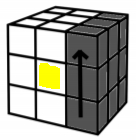
\includegraphics[width=0.3\linewidth]{images/move_3u}
\caption{Taking the nearer (highlighted) face as the frame of reference, this particular transformation would be described as a $[2,u]$ move. Using index notation, the third column of the face is rotated upwards by 90$^{\circ}$~\cite{proj_l.hoang}.}
\label{fig:fig2}
\end{small}
\end{figure}

This cube could be manipulated, as in Figure~\ref{fig:fig2} by an agent in order to reach a solution after a successful set of moves had been made.

\subsection{Results}

The following tables contain the mean runtime and the mean number of moves for solving both the Pocket Cube and Rubik's Cube, over what were considered idealised parameters.

\vspace{8pt}
{\centering
\resizebox{\linewidth}{!}{%
\begin{tabular}{||c||c|c|c|c|}
\hline
    $\text{n=2}$ & $\text{DRL + A}^{\ast}$ & \hspace{11pt} $\text{GA}$ \hspace{11pt}  & \hspace{11pt} $\text{SA}$ \hspace{11pt} & $\text{Baseline}$ \\
 \hline
 Runtime (s) & 3.1 & 0 & 0 & 10\\ %[0.5ex]
 \hline
 \# of Moves & 9.8 & 0 & 0 & 17\\
 \hline
\end{tabular}}

\vspace{8pt}
}

\vspace{8pt}
{\centering
\resizebox{\linewidth}{!}{%
\begin{tabular}{||c||c|c|c|c|}
\hline
    $\text{n=3}$ & $\text{DRL + A}^{\ast}$ & \hspace{11pt} $\text{GA}$ \hspace{11pt}  & \hspace{11pt} $\text{SA}$ \hspace{11pt} & $\text{Baseline}$ \\
 \hline
 Runtime (s) & 13.6 & 0 & 0 & 15\\ %[0.5ex]
 \hline
 \# of Moves & 22.1 & 0 & 0 & 32\\
 \hline
\end{tabular}}

\vspace{8pt}
}


% NOTE: COULD USE KORF AS A BASELINE
% TODO: Turn into table? Great idea!

\subsubsection{DRL + A$^{\ast}$}

\begin{figure}[!h]
\begin{small}
\centering
\linespread{1.0}
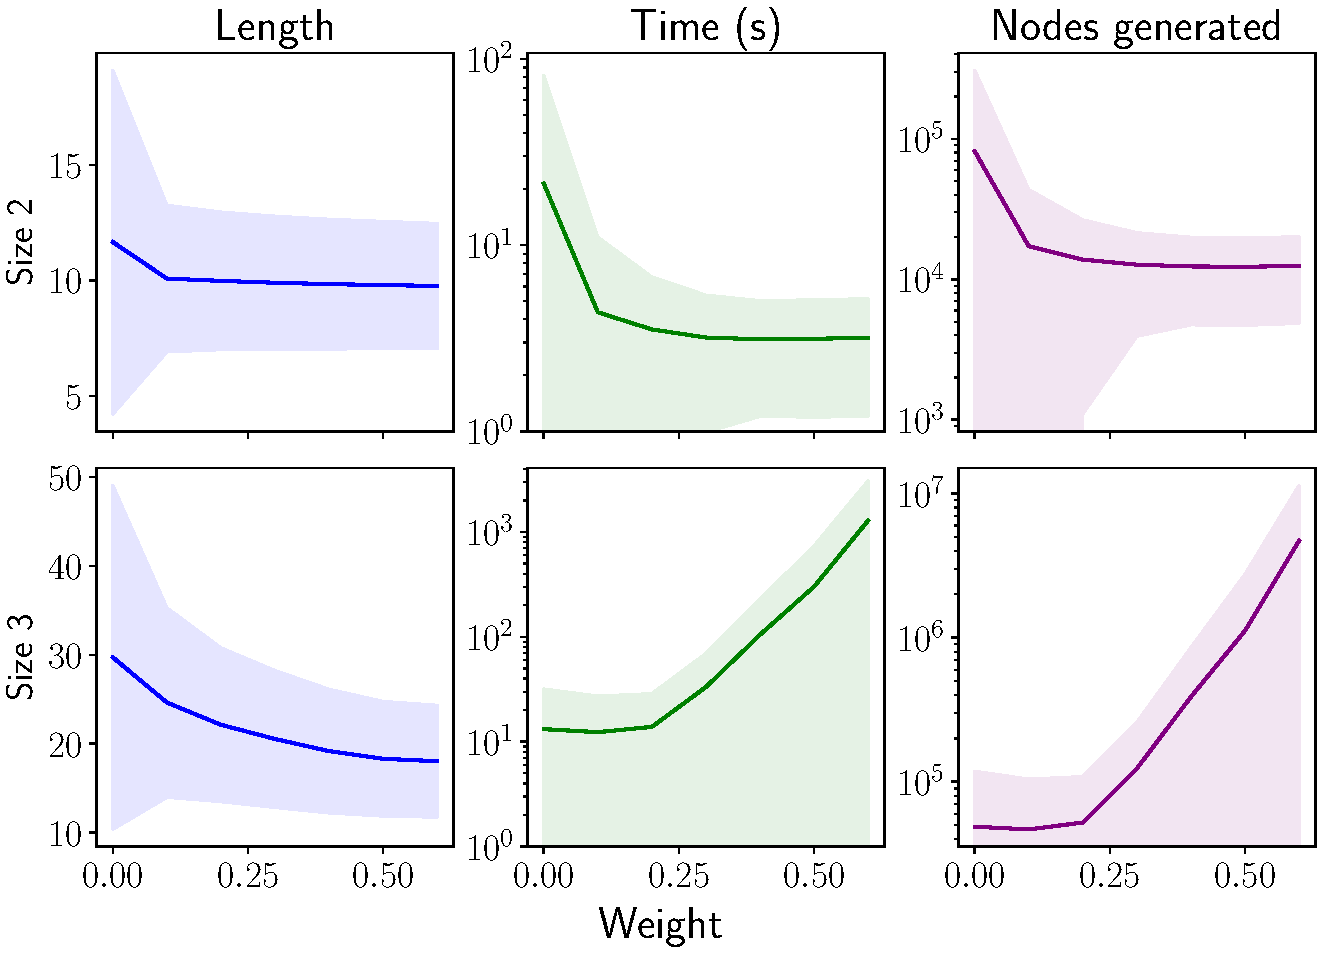
\includegraphics[width=0.75\linewidth]{images/bwas}
\caption{Employing Batch Weighted A$^{\ast}$ Search with a batch size of 100 (the number of nodes that can be expanded simultaneously), for cubes up to 100 randomised moves away from the goal state. The length of a solution is also known as the number of moves required to reach a solved state.}
\label{fig:fig3}
\end{small}
\end{figure}

\subsubsection{GA}


\subsubsection{SA}


\subsubsection{Baseline}

\subsection{Discussion}
It should be noted that the common metric used by the models, that is runtime and number of moves, immediately runs into a dilemma - should the DRL + A$^{\ast}$ model be evaluated only on the duration of the training or exclusively on the duration of the the solution of any given randomised cube. One could make the argument in either way, but highlighting that whilst the DRL + A$^{\ast}$ ran fastest, there was certainly a significant degree of overhead to its use.

Beyond that lay the parameters unique to each model, be it the number of layers for training the DNN, the A$^{\ast}$ weightings, the rate of mutation in the GA or the cooling rates in the SA. Modifying these values have well understood implications when the problems are treated in tandem - it is possible to see that in the case of GA and SA high mutation rates and high starting temperatures increase the time taken to arrive at a solution state, and yet such an analogous relationship does not exist for the DRL + A$^{\ast}$. However, one could (inelegantly) compare the number of generations in a GA with the number of layers in the NN used in the training process, arguing that many inputs are taken to ultimately return a unique item of use. According to present understanding, there is no such trait that can be described as truly common between the three methods employed in this investigation; where one analogy holds for two techniques, it either fails to capture the third outright or else makes the vaguest approximation to what is actually going on within the model.

\iffalse
This section should provide the details of the evaluation. Specifically:
\begin{itemize}
\item Methodology: describe the evaluation criteria, the data used during the evaluation, and the methodology followed to perform the evaluation. 
\item Results: present the results of the experimental evaluation. Graphical data and tables are two common ways to present the results. Also, a comparison with a baseline should be provided. 
\item Discussion: discuss the implication of the results of the proposed algorithms/models. What are the weakness/strengths of the method(s) compared with the other methods/baseline?
\end{itemize}
\fi

\section{Conclusions}
Provide a final discussion of the main results and conclusions of the report. Comment on the lesson learnt and possible improvements.


A standard and well formatted bibliography of papers cited in the report. For example:

\printbibliography
\end{document}

